%% IEEE ISEC 2027 -- K-12 poster extended abstract (max 2 pages, due Jan 31, 2027 via EDAS).
%% ISEC provides its own K-12 poster template: before uploading, copy this text into it
%% (https://ewh.ieee.org/conf/stem/author.html). This IEEEtran build is for drafting.
%% Compile this file instead of main.tex (Overleaf: Menu -> Main document).
\documentclass[conference]{IEEEtran}
\usepackage{cite,amsmath,graphicx,booktabs,xspace}
\usepackage[hidelinks]{hyperref}
\usepackage{xcolor}
\newcommand{\todo}[1]{\textcolor{red}{[TODO: #1]}}
\graphicspath{{figures/}}
% Auto-generated by scripts/make_figures.py. Do not edit.
\newcommand{\chainExcessHB}{0.089}
\newcommand{\chainExcessRatio}{1.5}
\newcommand{\chainExcessSeq}{0.132}
\newcommand{\chainHAGain}{-0}
\newcommand{\chainHBGain}{11}
\newcommand{\compFitRsq}{0.65}
\newcommand{\compFitSlope}{0.92}
\newcommand{\compHA}{22.5}
\newcommand{\compHB}{33.2}
\newcommand{\compHC}{25.1}
\newcommand{\compModular}{20.9}
\newcommand{\compParallel}{25.6}
\newcommand{\compRatioHB}{1.6}
\newcommand{\compSequential}{21.3}
\newcommand{\compSpeedupMax}{1.4}
\newcommand{\compSpeedupMin}{0.5}
\newcommand{\compSpread}{1.6}
\newcommand{\ctrlLatGap}{17}
\newcommand{\ctrlStepGap}{1}
\newcommand{\curvedConvHB}{4}
\newcommand{\curvedConvSeq}{8}
\newcommand{\curvedWallHB}{0.23}
\newcommand{\curvedWallRatio}{1.2}
\newcommand{\curvedWallSeq}{0.26}
\newcommand{\eagerSpread}{3.8}
\newcommand{\infChainHA}{0.094}
\newcommand{\infChainHB}{0.131}
\newcommand{\infChainHC}{0.067}
\newcommand{\infChainModular}{0.078}
\newcommand{\infChainParallel}{0.091}
\newcommand{\infChainSequential}{0.082}
\newcommand{\infCurvedHA}{0.093}
\newcommand{\infCurvedHB}{0.129}
\newcommand{\infCurvedHC}{0.067}
\newcommand{\infCurvedModular}{0.079}
\newcommand{\infCurvedParallel}{0.091}
\newcommand{\infCurvedSequential}{0.081}
\newcommand{\infLinearHA}{0.093}
\newcommand{\infLinearHB}{0.130}
\newcommand{\infLinearHC}{0.066}
\newcommand{\infLinearModular}{0.079}
\newcommand{\infLinearParallel}{0.091}
\newcommand{\infLinearSequential}{0.081}
\newcommand{\kernFitRsq}{0.99}
\newcommand{\latBigHA}{213}
\newcommand{\latBigHB}{322}
\newcommand{\latBigHC}{156}
\newcommand{\latBigModular}{193}
\newcommand{\latBigParallel}{314}
\newcommand{\latBigSequential}{196}
\newcommand{\latOneHA}{31.7}
\newcommand{\latOneHB}{38.2}
\newcommand{\latOneHC}{25.0}
\newcommand{\latOneModular}{10.0}
\newcommand{\latOneParallel}{16.1}
\newcommand{\latOneRatioHB}{3.3}
\newcommand{\latOneSequential}{11.7}
\newcommand{\longExcessRatio}{1.8}
\newcommand{\longHAGain}{-0}
\newcommand{\longHAThree}{0.345}
\newcommand{\longHBExcess}{0.051}
\newcommand{\longHBGain}{12}
\newcommand{\longHBPlateau}{227}
\newcommand{\longHBThree}{0.301}
\newcommand{\longHBpval}{0.005}
\newcommand{\longHBsig}{p<0.05}
\newcommand{\longParThree}{0.338}
\newcommand{\longSeqDrop}{10}
\newcommand{\longSeqExcess}{0.094}
\newcommand{\longSeqHundred}{0.382}
\newcommand{\longSeqPlateau}{270}
\newcommand{\longSeqThree}{0.344}
\newcommand{\modHA}{12}
\newcommand{\modHB}{13}
\newcommand{\modHC}{8}
\newcommand{\modModular}{3}
\newcommand{\modParallel}{4}
\newcommand{\modSequential}{5}
\newcommand{\mseChainHA}{0.383}
\newcommand{\mseChainHB}{0.339}
\newcommand{\mseChainHC}{0.378}
\newcommand{\mseChainModular}{0.382}
\newcommand{\mseChainParallel}{0.411}
\newcommand{\mseChainSequential}{0.382}
\newcommand{\mseCurvedHA}{3.987}
\newcommand{\mseCurvedHB}{4.029}
\newcommand{\mseCurvedHC}{3.994}
\newcommand{\mseCurvedModular}{4.045}
\newcommand{\mseCurvedParallel}{4.032}
\newcommand{\mseCurvedSequential}{4.045}
\newcommand{\mseLinearHA}{1.016}
\newcommand{\mseLinearHB}{1.027}
\newcommand{\mseLinearHC}{1.021}
\newcommand{\mseLinearModular}{1.022}
\newcommand{\mseLinearParallel}{1.023}
\newcommand{\mseLinearSequential}{1.022}
\newcommand{\opsFitRsq}{0.98}
\newcommand{\opsFitSlope}{2.8}
\newcommand{\opsHA}{10}
\newcommand{\opsHB}{13}
\newcommand{\opsHC}{8}
\newcommand{\opsModFitRsq}{0.998}
\newcommand{\opsModular}{3}
\newcommand{\opsParallel}{6}
\newcommand{\opsSequential}{3}
\newcommand{\perModUs}{1.0}
\newcommand{\perOpUs}{1.8}
\newcommand{\pilotSpeedup}{1.62}
\newcommand{\rtwoChainHA}{0.961}
\newcommand{\rtwoChainHB}{0.966}
\newcommand{\rtwoChainHC}{0.962}
\newcommand{\rtwoChainModular}{0.962}
\newcommand{\rtwoChainParallel}{0.959}
\newcommand{\rtwoChainSequential}{0.962}
\newcommand{\rtwoCurvedHA}{0.983}
\newcommand{\rtwoCurvedHB}{0.982}
\newcommand{\rtwoCurvedHC}{0.983}
\newcommand{\rtwoCurvedModular}{0.982}
\newcommand{\rtwoCurvedParallel}{0.982}
\newcommand{\rtwoCurvedSequential}{0.982}
\newcommand{\rtwoLinearHA}{0.971}
\newcommand{\rtwoLinearHB}{0.970}
\newcommand{\rtwoLinearHC}{0.970}
\newcommand{\rtwoLinearModular}{0.970}
\newcommand{\rtwoLinearParallel}{0.970}
\newcommand{\rtwoLinearSequential}{0.970}
\newcommand{\stepChainHA}{0.417}
\newcommand{\stepChainHB}{0.494}
\newcommand{\stepChainHC}{0.371}
\newcommand{\stepChainModular}{0.265}
\newcommand{\stepChainParallel}{0.328}
\newcommand{\stepChainSequential}{0.273}
\newcommand{\stepCurvedHA}{0.416}
\newcommand{\stepCurvedHB}{0.480}
\newcommand{\stepCurvedHC}{0.379}
\newcommand{\stepCurvedModular}{0.273}
\newcommand{\stepCurvedParallel}{0.326}
\newcommand{\stepCurvedSequential}{0.272}
\newcommand{\stepLinearHA}{0.425}
\newcommand{\stepLinearHB}{0.479}
\newcommand{\stepLinearHC}{0.372}
\newcommand{\stepLinearModular}{0.276}
\newcommand{\stepLinearParallel}{0.345}
\newcommand{\stepLinearSequential}{0.277}
\newcommand{\stepRatioHB}{1.81}
\newcommand{\threadHABigFour}{352}
\newcommand{\threadParallelFour}{179}
\newcommand{\threadParallelOne}{90}
\newcommand{\threadSeqBigFour}{146}
\newcommand{\torchVersion}{2.8.0}

\DeclareRobustCommand{\HB}{H\nobreakdash-B\xspace}

\begin{document}
\title{What a Student Benchmark Taught Me About Measuring Neural Network Speed}
\author{\IEEEauthorblockN{Aryan Kulkarni}
\IEEEauthorblockA{\textit{Bellarmine College Preparatory}, San Jose, CA, USA\\ aryanamol10@gmail.com}}
\maketitle

\begin{abstract}
As a high-school researcher, I compared sequential, parallel, modular, and hybrid neural networks on three
synthetic regression tasks. My first benchmark suggested that modular networks train
\pilotSpeedup$\times$ faster. An audit showed that this came from mixing two software frameworks and from
inputs that carried no information. A corrected, parameter-matched study with five random seeds found that how
parameters are wired changes inference latency far more than parameter count does, and that a modular
design matched to the problem's structure gave the best accuracy on the hardest task. I describe the project as
a case study in experimental rigor for pre-college computing research.
\end{abstract}

\section{Motivation}
Neural networks are often compared by parameter count, but users experience \emph{latency}. I asked:
with the same parameter budget, does arranging the parameters in sequence, in parallel, or as modules
change speed and accuracy?

\section{From a Flawed Pilot to a Fair Test}
The pilot used Keras for two models and PyTorch for the third. The ``fast'' modular model was mathematically
identical to the sequential one, so the speedup was the framework's, not the architecture's. Its training inputs
were also random numbers unrelated to the targets, so every model ended up predicting the average. The lesson
I took away was to change one variable at a time, hold out test data, repeat with several seeds, and include a
control that \emph{should} show no difference.

\section{Main Study}
Six models (about 385 parameters each) were trained in PyTorch on linear, curved, and chained functions,
with five seeds each. A latency sweep timed every model at batch sizes from 1 to 4096.

\begin{figure}[h]
\centering
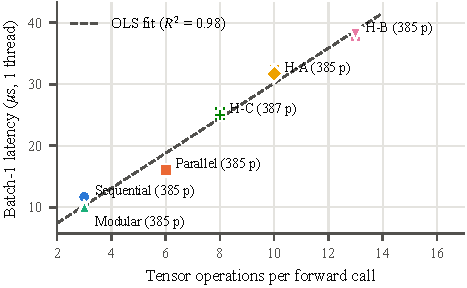
\includegraphics[width=\columnwidth]{fig_ops_latency}
\caption{Single-sample latency grows with the number of operations per call ($R^2=\opsFitRsq$), even though
every model has about the same number of parameters.}
\end{figure}

\section{Findings}
\begin{itemize}
\item On the chained task, the staged modular hybrid (\HB) reached test MSE \mseChainHB, compared with
\mseChainSequential\ for the plain sequential network.
\item \HB was also the slowest model at batch size 1 (\latOneHB\,\textmu s vs.\ \latOneSequential\,\textmu s),
because it runs the most operations per call.
\item Parameter count alone predicted neither speed nor accuracy.
\end{itemize}

\section{Reflection for STEM Education}
% ---------------------------------------------------------------------------------------------
% BLUEPRINT -- rewrite every sentence in your own voice. Judges value honesty and specifics.
% Aim for 4 short paragraphs (~200 words total). Fill in or delete each [bracketed] part.
%  1. The surprise:   the moment you realized the pilot result was wrong, and how it felt.
%  2. The lesson:     what "a fair comparison" means to you now (one variable at a time, controls).
%  3. The process:    one concrete skill you learned (seeds, held-out data, reading PyTorch docs...).
%  4. For others:     one piece of advice for a student starting their first ML project.
% ---------------------------------------------------------------------------------------------
\textbf{The surprise.} My first benchmark seemed to show that modular networks were
\pilotSpeedup$\times$ faster, and I [was ready to write it up / believed it at first]. The moment
I realized it was wrong was [describe it: e.g., noticing the ``fast'' model was mathematically
identical to the slow one]. [How did that feel, and what did you do next?]

\textbf{The lesson.} I learned that a fair comparison changes only one thing at a time. Mixing
two software frameworks meant I was measuring the frameworks, not the architectures. Now I
[plan a control that should show no difference / write down what I expect before running].

\textbf{The process.} The hardest new skill was [e.g., running five random seeds and reporting the
spread / holding out test data / reading the PyTorch source]. It mattered because [one sentence].

\textbf{For other students.} If I could tell another student one thing, it would be: [your advice].
Projects like this need no special hardware; every model here trains on a laptop.

\section*{Acknowledgment}
The pilot study used Google Colab. AI tools assisted with experiment code, figures, and drafting; the author
verified all content.

\end{document}
